\part Un péndulo alcanza una altura máxima $h$ relativa a la altura más baja mientras oscila. Podemos ignorar la fricción y la resistencia del aire.


\begin{figure}[H]
    \centering
    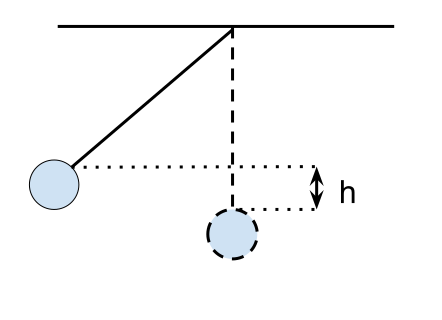
\includegraphics[width=0.5\linewidth]{../images/6f7b57146c85d8c1c8e1fbce4d78a2d3c2fcac2a}
\end{figure}
\textbf{¿Dónde está el péndulo cuando tiene la mínima energía potencial?}

\begin{choices}
    \CorrectChoice En la altura mínima
    \choice En la altura máxima
    \choice Es la misma a lo largo de su movimiento
    \choice No hay suficiente información
\end{choices}

\textbf{¿Dónde está el péndulo cuando tiene la máxima energía potencial?}

\begin{choices}
    \choice En la altura mínima
    \CorrectChoice En la altura máxima
    \choice Es la misma a lo largo de su movimiento
    \choice No hay suficiente información
\end{choices}

\textbf{¿Dónde está el péndulo cuando tiene la mínima energía cinética?}

\begin{choices}
    \choice En la altura mínima
    \CorrectChoice En la altura máxima
    \choice Es la misma a lo largo de su movimiento
    \choice No hay suficiente información
\end{choices}
\textbf{¿Dónde está el péndulo cuando tiene la máxima energía cinética?}

\begin{choices}
    \CorrectChoice En la altura mínima
    \choice En la altura máxima
    \choice Es la misma a lo largo de su movimiento
    \choice No hay suficiente información
\end{choices}


